
\begin{frame}[ctb!]
  \frametitle{Proposal : A Proof of Concept} 

  Proof of concept work was developed and implemented in three phases:

  \begin{enumerate}
    \item development of a proof of concept specification language for dynamic
      fuel cycles
    \item implementation of the specification for (simple) once-through base
      cases in both the INPRO and NEA/OECD benchmarks
    \item translation of the implementation into a Cyclus input file, and
      subsequently running the simulation
  \end{enumerate}

  \pause
  
  We highlight the fact that:

  \begin{itemize}
    \item this is a suggestion, not a complete solution
    \item there are definitely things missing from a full specification
    \item we see this as a starting point to begin a more community-wide
      discussion on how to address this issue
  \end{itemize}
\end{frame}

\begin{frame}[fragile]
  \frametitle{Proposal : Basic Language Structure}
  \begin{columns}[t]
    \column{.5\textwidth}\begin{block}{Specification}\begin{small}\begin{verbatim}
* materials
  * aMaterial
    * metadata
    * attributes
    * constraints
      
* facilities
  * aFacility
    * metadata
    * attributes
    * constraints
      
* fuelCycle
  * metadata
  * attributes
  * constraints
    \end{verbatim}\end{small}\end{block}
    \column{.5\textwidth}\begin{block}{JSON Implementation}\begin{small}\begin{verbatim}
{"materials":     
  "metadata": {},
  "attributes": {},
  "constraints": {}
},
      
{"facilities":     
  "metadata": {},
  "attributes": {},
  "constraints": {}
},

{"fuelCycle":     
  "metadata": {},
  "attributes": {},
  "constraints": {}
}
      \end{verbatim}\end{small}\end{block}
  \end{columns}
\end{frame}

\begin{frame}[fragile]
  \frametitle{Proposal : Materials}
  \begin{columns}[t]
    \column{.5\textwidth}\begin{block}{Specification}\begin{small}\begin{verbatim}
* materials
  * name1
    * metadata (optional)
      * suggestedComposition (optional)
        * isotope1
        * isotope2
      * attributes
        * recipe
          * true/false
        * parents (optional)
      * constraints
        * constraint1
        * constraint2...
  * name2...
    \end{verbatim}\end{small}\end{block}
    \column{.5\textwidth}\begin{block}{JSON Implementation}\begin{small}\begin{semiverbatim}
\only<1>{\{"materials":    
    "leu": \{
      "attributes": \{
        "recipe": true
      \},
      "constraints": [      
        ["U235", 0.0495],
        ["U238", 0.9505],
        ["O16", 2.0],
        ["density", 10.2]
      ]
  \},
}
\only<2>{"spent_pwr_uox": \{
      "metadata": \{
        "suggestedComposition": [
          ["U235",0.02],
          ...
        ]
      \},
      "attributes": \{
        "recipe": false
      \},
      "constraints": [
        "id == 92235 && x < 0.0495",
        "id == 92238 && x < 0.9505",
        "density < 10.2"
      ]
  \}
\}
}
      \end{semiverbatim}\end{small}\end{block}
  \end{columns}
\end{frame}

\begin{frame}[fragile]
  \frametitle{Proposal : Facilities - Reactor}
  \begin{columns}[t]
    \column{.5\textwidth}\begin{block}{Specification}\begin{footnotesize}\begin{semiverbatim}
\only<1>{* name
* metadata (optional)
  * type: reactor
* attributes
  * thermalPower: units
  * efficiency: units
  * cycleLegth: units
  * capacityFactor: units 
  * lifetime: \{units | distributed\} 
  * fuelTypes: fuel1, fuel2..
  * batches: units, fuelTypes
  * coreLoading: units, fuelTypes
  * burnup: units, fuelTypes
  * coolingTime: units, fuelTypes
  * storageTime: units, fuelTypes
}
\only<2>{* constraints
  * thermalPower: value
  * efficiency: value
  * cycleLegth: value
  * capacityFactor: value 
  * batches: value
  * lifetime: \{value | distributed\}
  * batches: value, fuelType
  * coreLoading: value, fuelType
  * burnup: value, fuelType
  * coolingTime: value, fuelType
  * storageTime: value, fuelType
* inputMaterials
* outputMaterials
}
    \end{semiverbatim}\end{footnotesize}\end{block}
    \column{.5\textwidth}\begin{block}{JSON Implementation}\begin{footnotesize}\begin{semiverbatim}
\only<1>{"lwr_reactor": \{
  "metadata": \{
    "type":"reactor"
  \},
  "attributes": \{
    "thermalPower": ["float", "GWt"],
    "efficiency": ["float", "percent"],
    "cycleLength": ["int", "month"],
    "lifetime": ["int", "year"],
    "fuels": ["leu"],
    "batches": ["int", "", ["leu"]],
    "coreLoading": ["float", "kg", ["leu"]],
    "burnup": ["float", "GWd/tHM", ["leu"]],
    "storageTime": ["int", "year", ["leu"]],
    "coolingTime": ["int", "year", ["leu"]],
  \},
}
\only<2>{  "constraints": [
    ["thermalPower", 4.25],
    ["efficiency", 34.1],
    ["cycleLength", 12],
    ["lifetime", 60],
    ["batches", 3, "leu"],
    ["coreLoading", 78.7, "leu"],
    ["burnup", 60, "leu"],
    ["storageTime", 2, "leu"],
    ["coolingTime", 5, "leu"]
  ],
  "inputMaterials": ["leu"],
  "outputMaterials": ["used_leu"]
\}
}
    \end{semiverbatim}\end{footnotesize}\end{block}
  \end{columns}
\end{frame}

\begin{frame}[fragile]
  \frametitle{Proposal : Facilities - Repositories}
  \begin{columns}[t]
    \column{.5\textwidth}\begin{block}{Specification}\begin{small}\begin{semiverbatim}
* name
  * metadata (optional)
    * type: repository
  * attributes
    * capacity: units
    * lifetime: units
  * constraints
    * capacity: value
    * lifetime: value
  * inputMaterials
    \end{semiverbatim}\end{small}\end{block}
    \column{.5\textwidth}\begin{block}{JSON Implementation}\begin{small}\begin{semiverbatim}
"lwr_repository": \{
  "metadata: \{
    "type":"repository"
  \},
  "attributes": \{
    "lifetime": ["int", "year"], 
    "capacity": ["double", "tHM/year"]
  \},
  "constraints": [
    ["lifetime", 60], 
    ["capacity", 800.0]
   ], 
 "inputMaterials": ["used_leu"]
\}
    \end{semiverbatim}\end{small}\end{block}
  \end{columns}
\end{frame}

\begin{frame}[fragile]
  \frametitle{Proposal : Facilities - Enrichment}
  \begin{columns}[t]
    \column{.5\textwidth}\begin{block}{Specification}\begin{footnotesize}\begin{semiverbatim}
* name
  * metadata (optional)
    * type: enrichment
  * attributes
    * capacity: units
    * lifetime: units
    * tailsFraction: units
  * constraints
    * capacity: value
    * lifetime: value
    * tailsFraction: value
  * inputMaterials
  * outputMaterials
    \end{semiverbatim}\end{footnotesize}\end{block}
    \column{.5\textwidth}\begin{block}{JSON Implementation}\begin{footnotesize}\begin{semiverbatim}
"lwr_enrichment": \{
  "metadata: \{
    "type":"enrichment"
  \},
  "attributes": \{
    "lifetime": ["int", "year"], 
    "capacity": ["double", "SWU/year"],
    "tailsFraction": ["double", 
                      "weight percent"]
  \},
  "constraints": [
    ["lifetime", 60], 
    ["capacity", 1e5],
    ["tailsFraction", 0.03]
  ], 
  "inputMaterials": ["natl_u"],
  "outputMaterials": ["leu", "tails"]
\}
    \end{semiverbatim}\end{footnotesize}\end{block}
  \end{columns}
\end{frame}


\begin{frame}[fragile]
  \frametitle{Proposal : Fuel Cycle Description}
  \begin{columns}[t]
    \column{.5\textwidth}\begin{block}{Specification}\begin{small}\begin{semiverbatim}
\only<1>{* fuelCycle
  * metadata (optional)
  * attributes
    * grid: units
    * initialConditions:
      * facility1: number
      * facility2...
    * demands:
      * demand1: units, facilities
      * demand2...
}
\only<2>{  * constraints
    * grid: value
    * demand1:
      * grid: value
      * growth:
        * type: growthType
        * period1: 
          * startTime: value
          * startValue: value
          * slope: value
        * period2...
    * demand2...
  * availableTechnologies (optional)
    * technology: period
}
    \end{semiverbatim}\end{small}\end{block}
    \column{.5\textwidth}\begin{block}{JSON Implementation}\begin{small}\begin{semiverbatim}
\only<1>{"fuelCycle": \{
  "attributes": \{
    "grid": "year",
    "initialConditions": \{
      "repository": 1,
    \},
    "demands": \{
      "power": [
               "GWe", 
               ["lwrReactor"]
      ]
    \}
  \}
}
\only<2>{  "constraints": \{
   "grid": [0, 120],
     "demands": \{
       "power": \{
         "grid": [0,120],
         "growth": \{
           "type": "linear",
           "period1": \{
             "startTime": 0,
             "startValue": 1000,
             "slope": 500
           \}
         \}
       \}
     \}
  \}
}
    \end{semiverbatim}\end{small}\end{block}
  \end{columns}
\end{frame}

\begin{frame}[fragile]
  \frametitle{Proposal : INPRO Once Through}
  \begin{figure}
    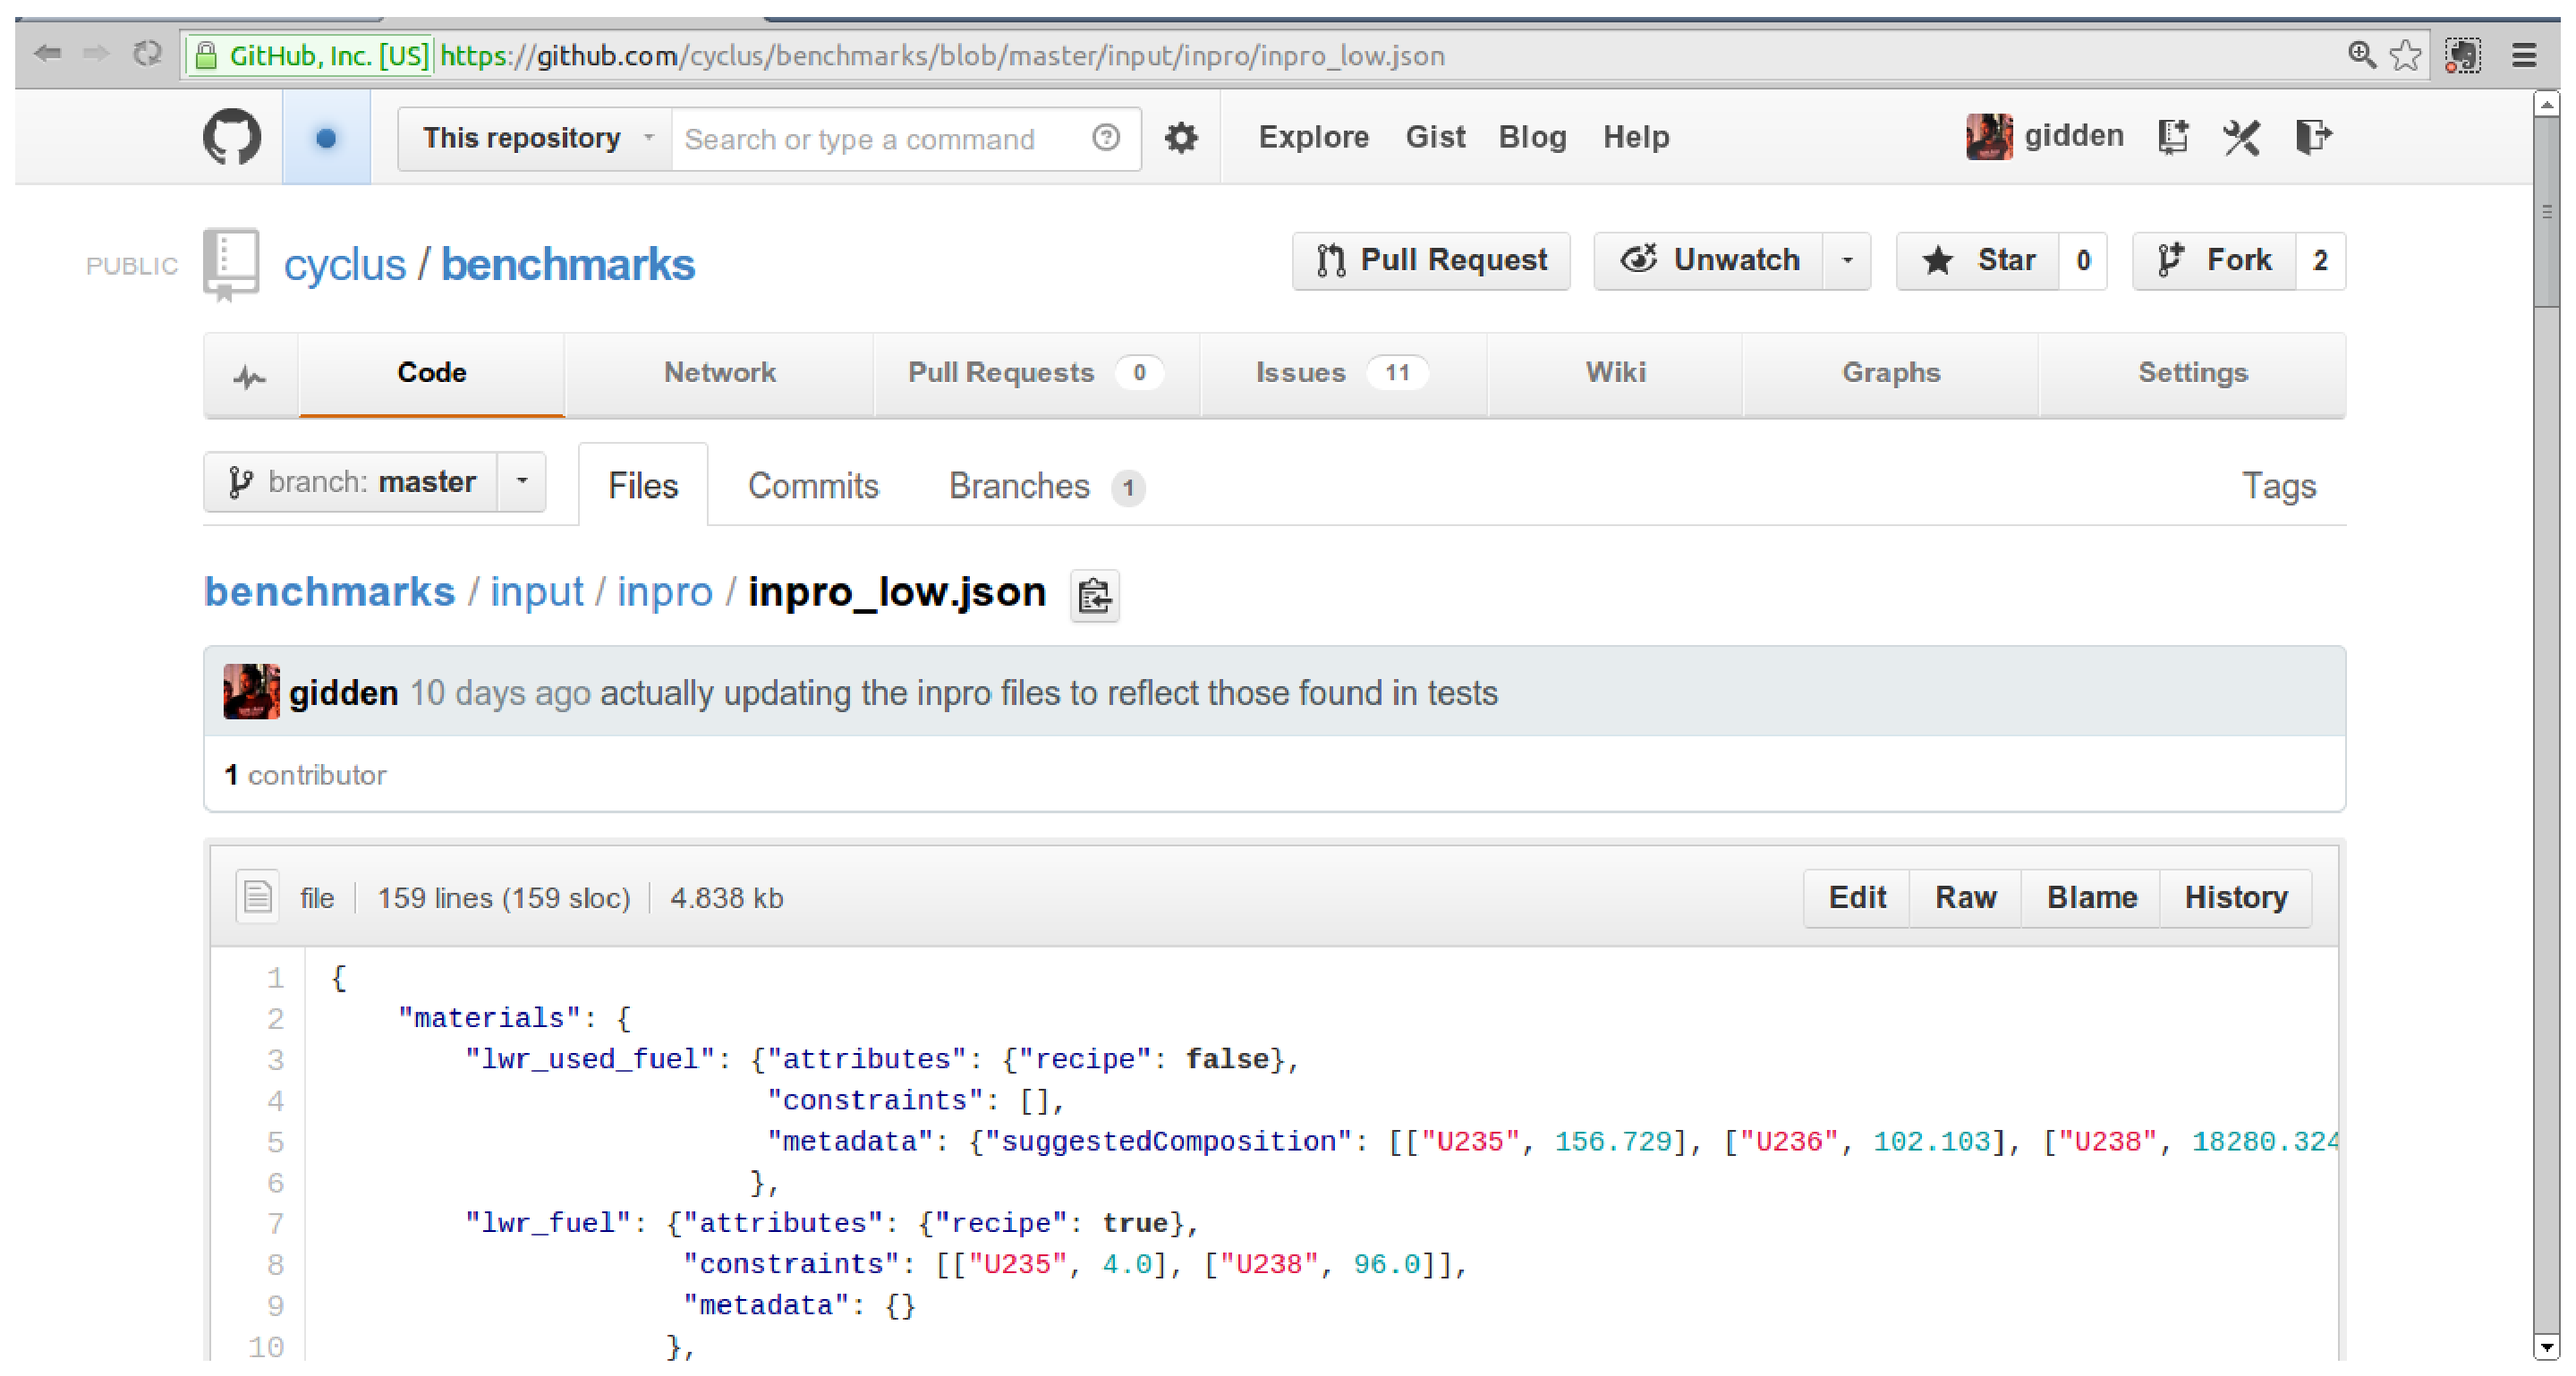
\includegraphics[width=\linewidth, height=\textheight, keepaspectratio]{inpro.eps}
    \caption{A Screenshot of the INPRO JSON File.}
  \end{figure}
\end{frame}

\begin{frame}[fragile, label = current]
  \frametitle{Proposal : NEA Once Through}
  \begin{figure}
    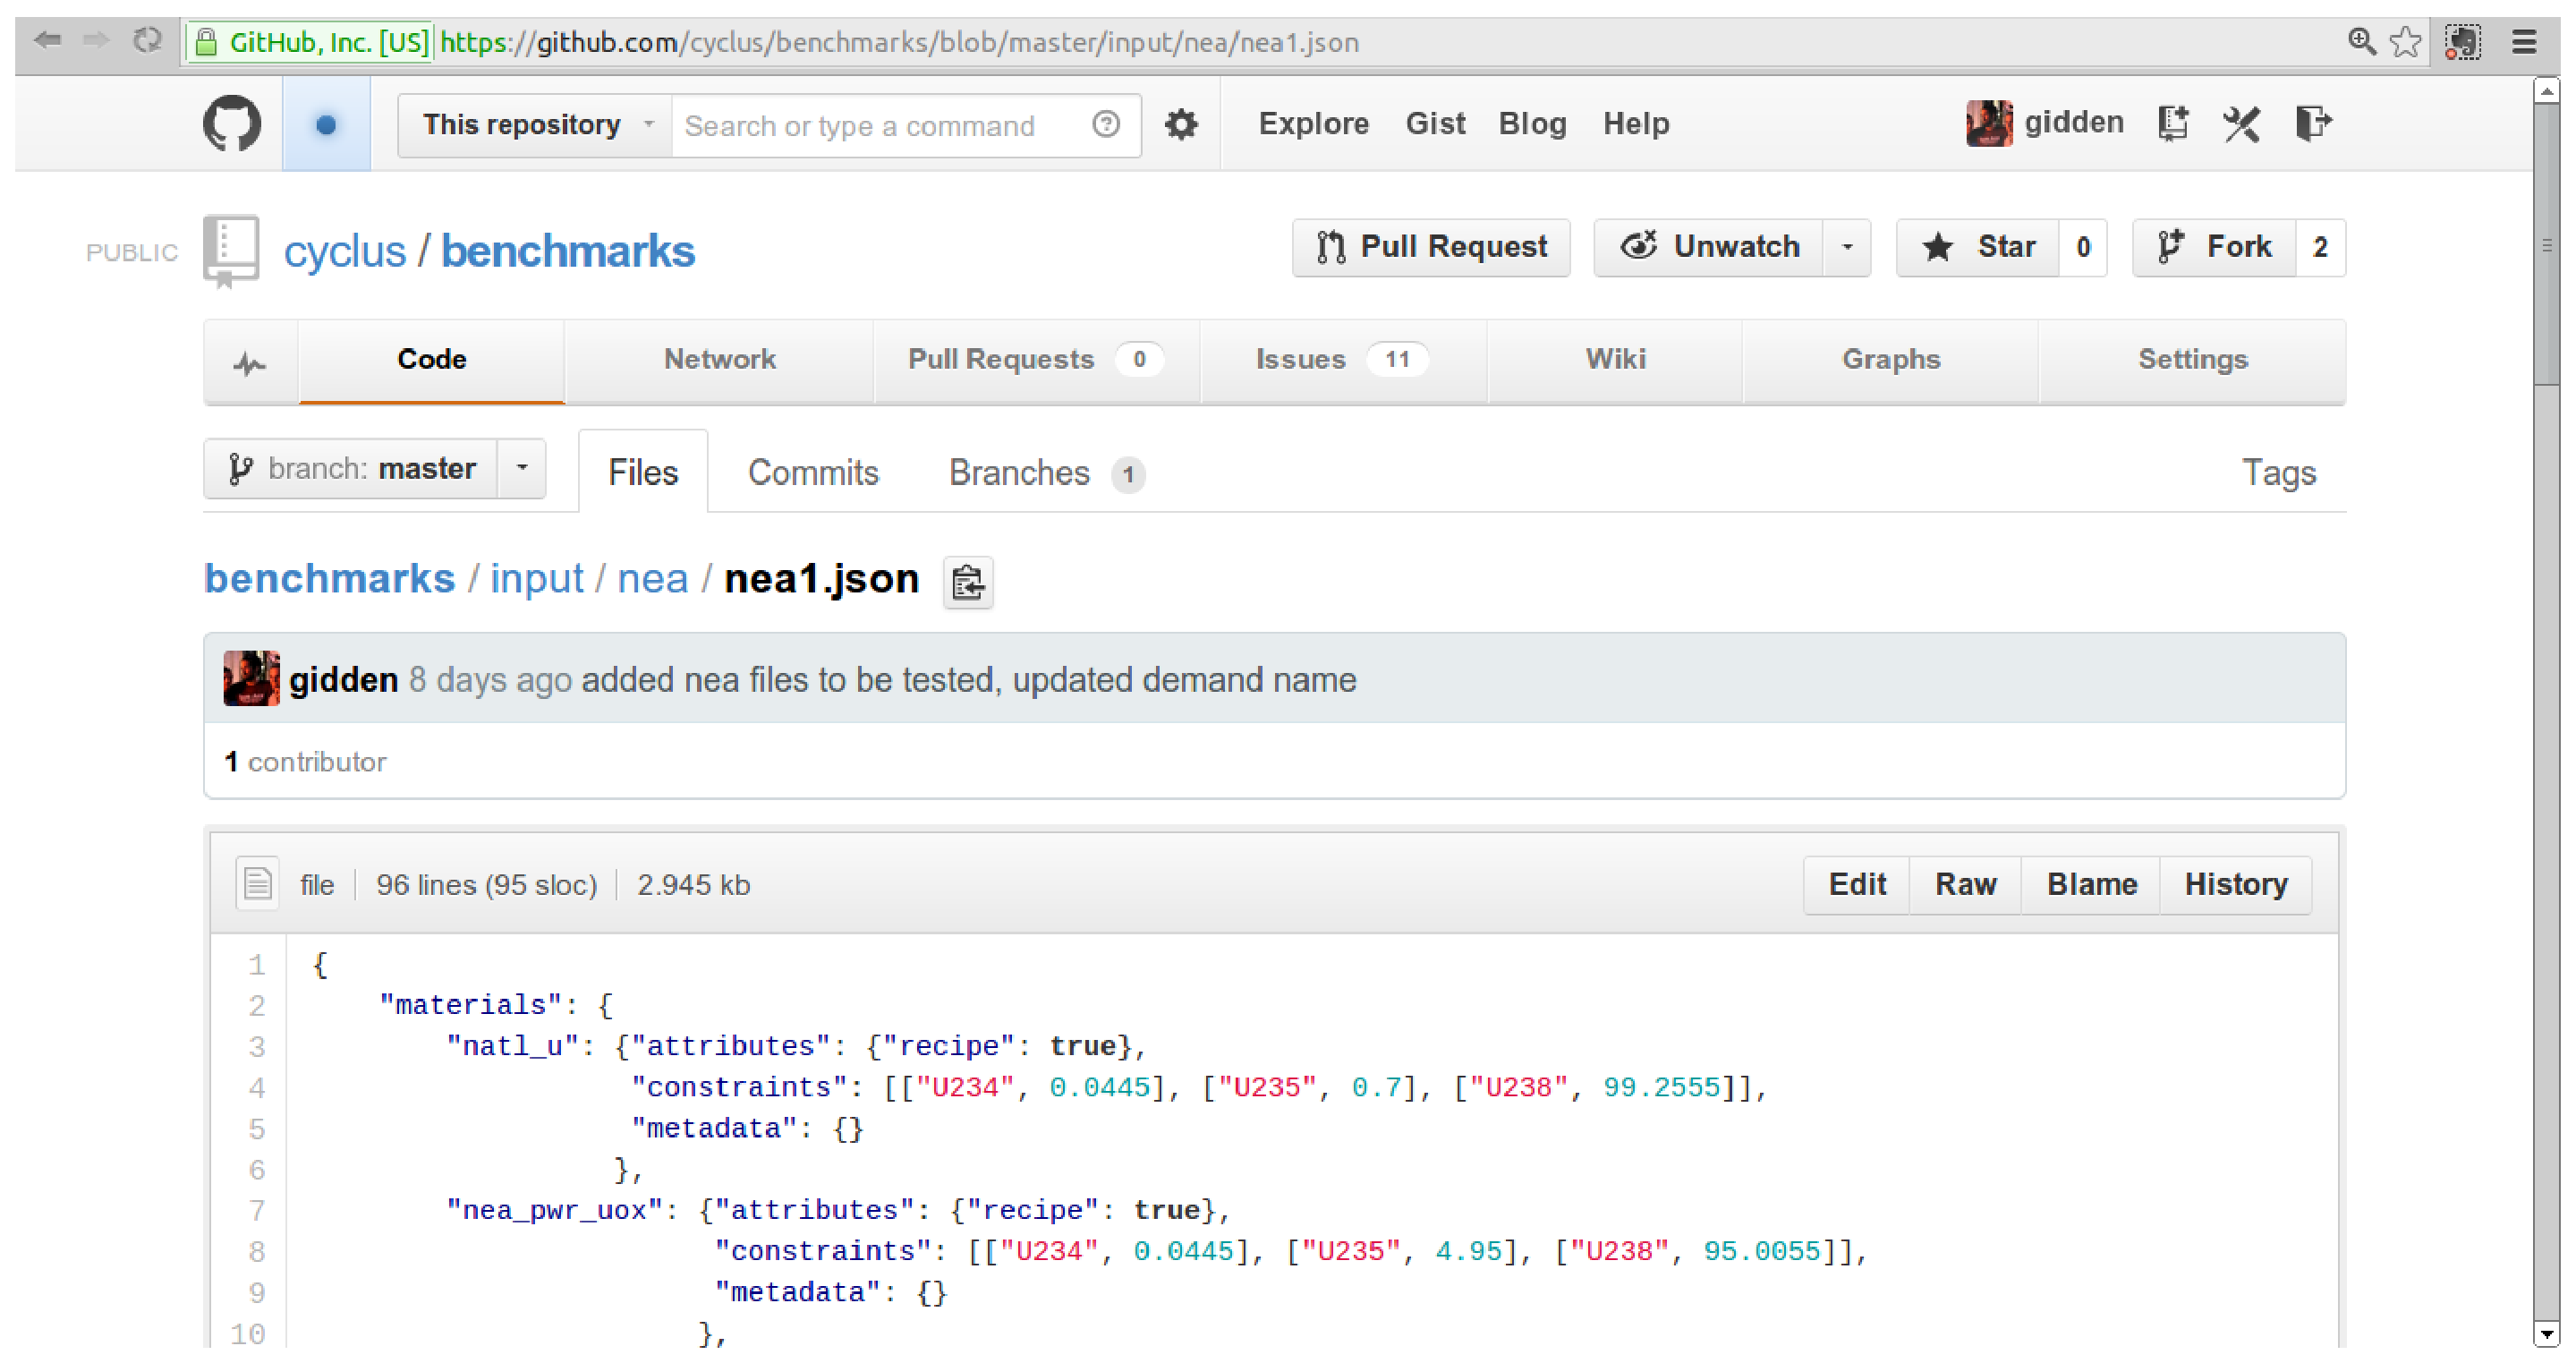
\includegraphics[width=\linewidth, height=\textheight, keepaspectratio]{nea.eps}
    \caption{A Screenshot of the NEA JSON File.}
  \end{figure}
\end{frame}
